\chapter{Subgroup symmetry as a resolved object}
\label{ch:subgroup-resolution}

The recovered Resolution Theory manuscript develops a direction that is both useful and exact. Once a finite group action has been supplied, subgroup invariants become ranges of averaging projectors. Inclusion, compatibility, and normality can then be read in an operator language. This chapter reconstructs that direction with proofs in the regular representation. The construction works for every finite group. Its input is the group, rather than a field over \(\Q\) having that group as its Galois group.

That distinction matters because the regular representation is available before any arithmetic realization has been found. It is a complete place to test the proposed subgroup calculus. An arithmetic extension, when one exists, can be translated into this language. Recovering the arithmetic extension from an arbitrary projector family requires more data, including multiplication and its descent to the desired base field.

\section{The regular module and its fixed ranges}

Let \(G\) be a finite group. Write \(V=\C[G]\) for the vector space with orthonormal basis \(\{\delta_g:g\in G\}\). The left regular action is
\begin{equation}
 \lambda(a)\delta_g=\delta_{ag}.
 \label{eq:b-regular-action}
\end{equation}
Every \(\lambda(a)\) is unitary. Extend \(\lambda\) linearly to the group algebra. This extension is injective, since
\begin{equation}
 \lambda\!\left(\sum_{g\in G}c_g g\right)\delta_1
 =\sum_{g\in G}c_g\delta_g.
 \label{eq:b-regular-faithfulness}
\end{equation}
Equality of regular operators therefore gives equality of all group algebra coefficients. This stronger property will justify the reverse implications below.

For \(H\leq G\), define
\begin{equation}
 e_H=\frac1{|H|}\sum_{h\in H}h\in\C[G],
 \qquad
 E_H=\lambda(e_H)=\frac1{|H|}\sum_{h\in H}\lambda(h).
 \label{eq:b-subgroup-average}
\end{equation}
The notation \(E_H\) in this chapter and its figures always means this operator. It is an average with normalization \(1/|H|\), rather than an unnormalized sum.

\begin{theorem}[Fixed range and rank]
\label{thm:b-fixed-range}
The operator \(E_H\) is the orthogonal projector onto
\[
 V^H=\{v\in V:\lambda(h)v=v\text{ for every }h\in H\}.
\]
Its rank is \([G:H]\). If \(H\leq K\), then
\begin{equation}
 E_HE_K=E_KE_H=E_K,
 \qquad V^K\subseteq V^H.
 \label{eq:b-nested-averages}
\end{equation}
\end{theorem}

\begin{proof}
Inversion permutes the elements of \(H\), so \(E_H^*=E_H\). Every element \(u\in H\) occurs exactly \(|H|\) times among the products \(hk\) with \(h,k\in H\). Consequently
\[
 E_H^2=\frac1{|H|^2}\sum_{h,k\in H}\lambda(hk)
 =\frac1{|H|}\sum_{u\in H}\lambda(u)=E_H.
\]
For \(a\in H\), left multiplication permutes the terms in the average, giving \(\lambda(a)E_H=E_H\). Thus its range consists of fixed vectors. Conversely, an \(H\) fixed vector is unchanged by every summand, and therefore by the average.

The orbits of \(H\) on the basis labels are the right cosets \(Hg\). For one representative \(g\) from each coset, put
\[
 v_{Hg}=|H|^{-1/2}\sum_{h\in H}\delta_{hg}.
\]
These vectors have disjoint supports, are orthonormal, and span the fixed range. Their number is \([G:H]\). Finally \(H\leq K\) makes every \(K\) fixed vector \(H\) fixed. Orthogonal projectors onto nested subspaces multiply to the projector onto the smaller subspace, in either order. This proves \eqref{eq:b-nested-averages}.
\end{proof}

In particular, the identity subgroup gives \(E_{\{1\}}=I\), while the whole group gives a rank one projector onto the constant vector. Every intermediate subgroup supplies a resolution \(\{E_H,I-E_H\}\). The word resolution here refers to the vector space decomposition into fixed vectors and their orthogonal complement. A field structure has not been imposed on these ranges.

The subgroup itself can be recovered from its regular average: the nonzero coefficients of \(E_H\delta_1\) have precisely the labels in \(H\). Thus distinct subgroups give distinct operators, including subgroups having the same order and the same projector rank. Rank by itself remembers the index, while the labelled operator remembers more.

\begin{figure}[tbp]
\centering
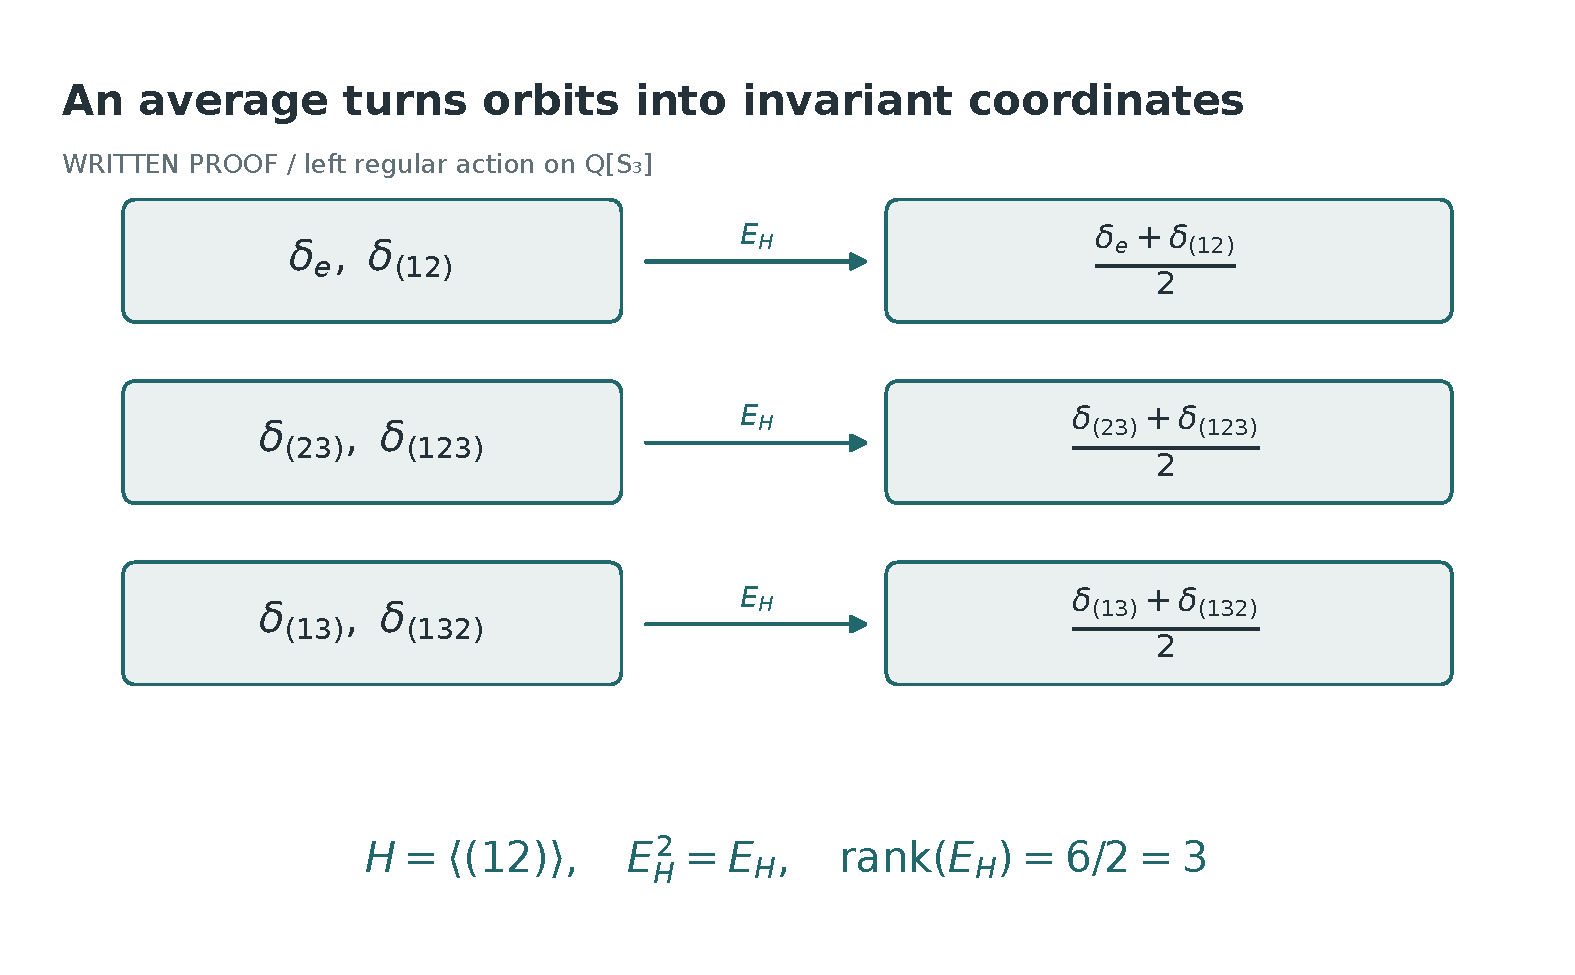
\includegraphics[width=0.96\linewidth]{../visual/figures/11_subgroup_projector.pdf}
\caption{The orbits of a subgroup's left action are the right cosets \(Hg\). Averaging replaces each orbit by one fixed vector, giving rank \([G:H]\). Enlarging the subgroup reduces the fixed range.}
\label{fig:b-subgroup-projector}
\end{figure}

\section{Products and the compatibility boundary}

For subgroups \(H,K\), the set \(HK=\{hk:h\in H,k\in K\}\) need not be a subgroup. The condition \(HK=KH\) is called permutability. It concerns the two product sets, and does not mean that every element of \(H\) commutes with every element of \(K\).

\begin{lemma}[Uniform product multiplicity]
\label{lem:b-product-multiplicity}
Every element of \(HK\) has exactly \(|H\cap K|\) expressions as \(hk\). Hence
\begin{equation}
 |HK|=\frac{|H||K|}{|H\cap K|},
 \qquad
 e_He_K=\frac1{|HK|}\sum_{x\in HK}x.
 \label{eq:b-product-support}
\end{equation}
The last sum is defined even when \(HK\) is not a subgroup.
\end{lemma}

\begin{proof}
Fix one expression \(x=h_0k_0\). An equality \(hk=h_0k_0\) is equivalent to \(h_0^{-1}h=k_0k^{-1}\in H\cap K\). For each \(a\in H\cap K\), the pair \((h_0a,a^{-1}k_0)\) gives one expression. This is a bijection. Counting all pairs proves the cardinality formula, and counting their coefficients in the group algebra proves the second identity.
\end{proof}

\begin{theorem}[Exact compatibility criterion]
\label{thm:b-compatible-averages}
In the regular realization, the following statements are equivalent:
\[
 HK=KH,\qquad HK\text{ is a subgroup},\qquad E_HE_K=E_KE_H.
\]
When they hold,
\begin{equation}
 E_HE_K=E_KE_H=E_{HK}=E_{\langle H,K\rangle}.
 \label{eq:b-compatible-product}
\end{equation}
Without a compatibility assumption, the intersection of the fixed ranges is still
\begin{equation}
 V^H\cap V^K=V^{\langle H,K\rangle}.
 \label{eq:b-fixed-intersection}
\end{equation}
\end{theorem}

\begin{proof}
If \(HK=KH\), then products of two elements of \(HK\) stay in \(HK\), because the middle factors can be written in the other order. Inversion sends \(HK\) to \(KH=HK\), and the identity belongs to it. It is therefore a subgroup. Conversely, if \(HK\) is a subgroup, its inverse set is itself, so \(KH=(HK)^{-1}=HK\).

For permutable subgroups, \eqref{eq:b-product-support} gives \(e_He_K=e_{HK}=e_Ke_H\). Applying \(\lambda\) proves the operator equality. If the operators commute, injectivity in \eqref{eq:b-regular-faithfulness} gives \(e_He_K=e_Ke_H\). Their supports are \(HK\) and \(KH\), with positive coefficients, so the sets are equal. A subgroup \(HK\) contains both \(H\) and \(K\), and is contained in every subgroup containing both, hence equals \(\langle H,K\rangle\). Finally, a vector fixed by both groups is fixed by every word in their elements and inverses. This proves the intersection identity without requiring their averages to commute.
\end{proof}

There is also an exact projector test. If \(P,Q\) are orthogonal projections and \(PQ\) is an orthogonal projection, then self adjointness gives \(PQ=(PQ)^*=QP\). In the compatible case, \(E_HE_K\) is the projection onto the common fixed range. In the incompatible case, one must retain the ordered products as transfers. Replacing them by a shared refinement would remove a real commutator.

\begin{example}[Two transpositions in \(S_3\)]
\label{ex:b-s3-incompatibility}
Let \(a=(12)\), \(b=(23)\), \(r=(123)\), and use permutation composition from right to left. Put \(H=\{1,a\}\), \(K=\{1,b\}\). Then \(ab=r\), \(ba=r^{-1}\), so
\[
 E_HE_K\delta_1=\tfrac14(\delta_1+\delta_a+\delta_b+\delta_r),
 \qquad
 E_KE_H\delta_1=\tfrac14(\delta_1+\delta_a+\delta_b+\delta_{r^{-1}}).
\]
In particular,
\begin{equation}
 [E_H,E_K]\delta_1
 =\tfrac14(\delta_r-\delta_{r^{-1}})\ne0.
 \label{eq:b-s3-commutator}
\end{equation}
Each average has rank three. Their common fixed range has rank one, because \(a,b\) generate \(S_3\). The rank one projector onto that intersection exists, even though it is not their ordered product.
\end{example}

For the figures we order the basis as
\[
 1,(12),(23),(13),(123),(132).
\]
The matrices of the two averages in this order are
\begin{equation}
 E_H=\frac12
 \begin{pmatrix}
 1&1&0&0&0&0\\
 1&1&0&0&0&0\\
 0&0&1&0&1&0\\
 0&0&0&1&0&1\\
 0&0&1&0&1&0\\
 0&0&0&1&0&1
 \end{pmatrix},
 \quad
 E_K=\frac12
 \begin{pmatrix}
 1&0&1&0&0&0\\
 0&1&0&0&0&1\\
 1&0&1&0&0&0\\
 0&0&0&1&1&0\\
 0&0&0&1&1&0\\
 0&1&0&0&0&1
 \end{pmatrix}.
 \label{eq:b-s3-matrices}
\end{equation}
The six columns of their commutator each have two entries of magnitude \(1/4\). Thus its squared Hilbert Schmidt norm is \(6\cdot2/16=3/4\). The exact computation bundle checks these matrices and all thirty six ordered pairs of subgroups of \(S_3\). Those finite checks confirm the worked example. The proof of Theorem~\ref{thm:b-compatible-averages} supplies the statement for arbitrary finite groups.

\begin{figure}[tbp]
\centering
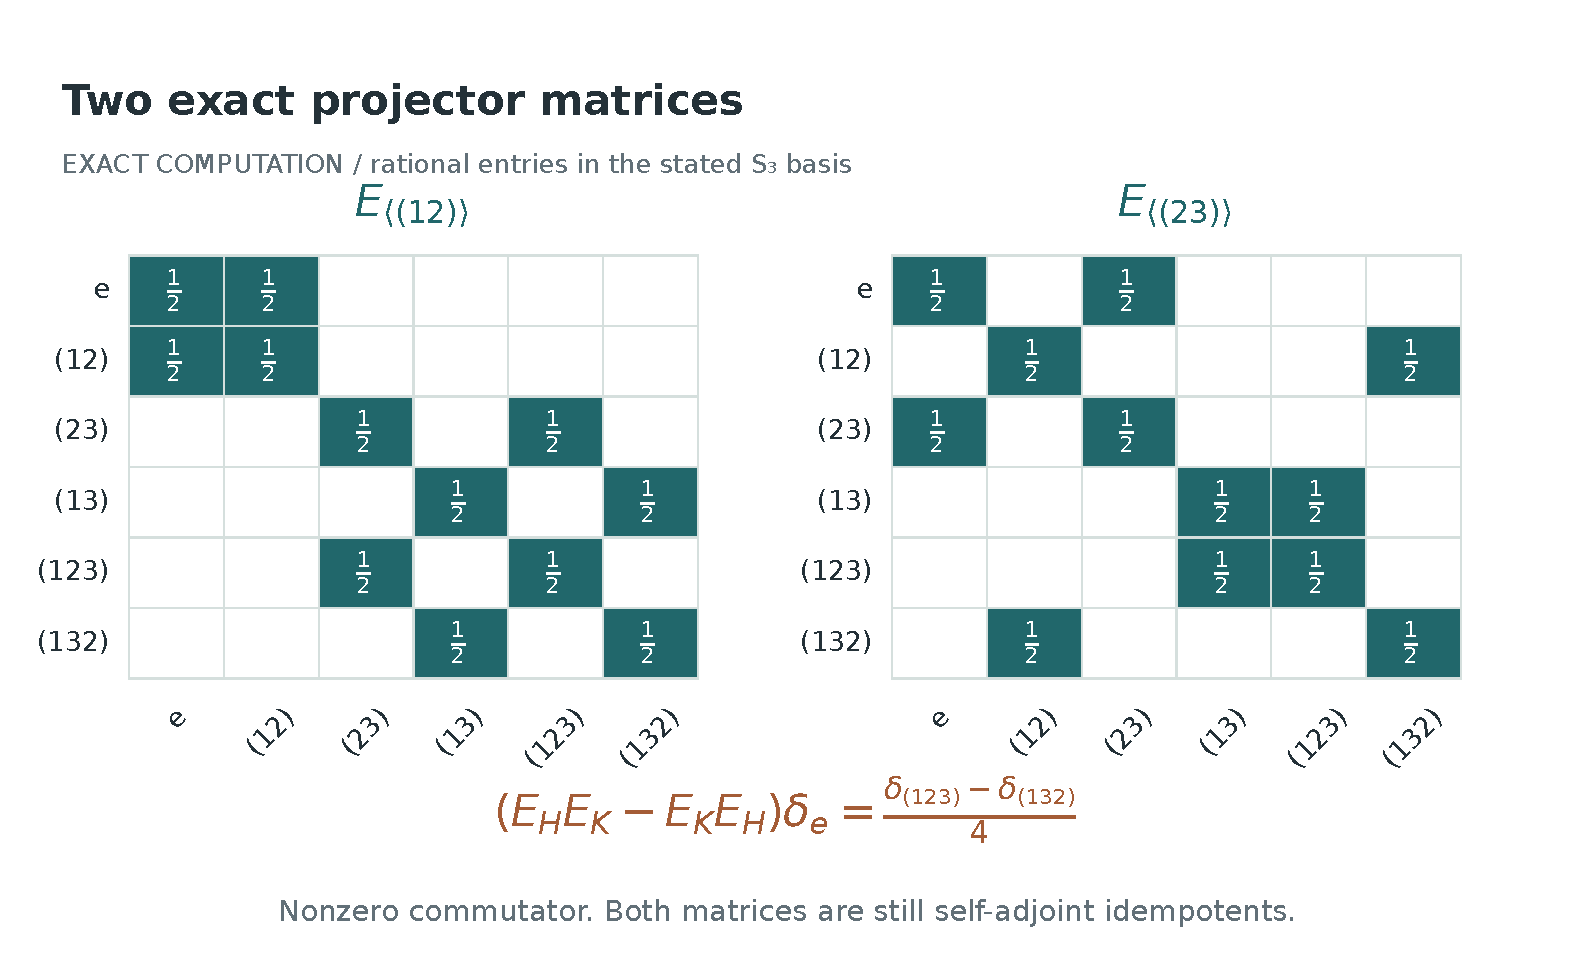
\includegraphics[width=0.96\linewidth]{../visual/figures/12_s3_matrix.pdf}
\caption{Exact \(S_3\) subgroup averages in the declared basis order. The displayed matrices are rational, and the nonzero commutator has squared Hilbert Schmidt norm \(3/4\).}
\label{fig:b-s3-matrix}
\end{figure}

\Needspace{14\baselineskip}
\section{Normality and the meaning of faithful realization}

\begin{theorem}[Normality as central compatibility]
\label{thm:b-normality}
For \(H\leq G\), the following are equivalent in the regular realization:
\begin{enumerate}
\item \(H\) is normal in \(G\).
\item \(e_H\) belongs to the center of \(\C[G]\).
\item \(E_H\) commutes with every \(\lambda(g)\).
\item \(V^H\) is invariant under every \(\lambda(g)\).
\end{enumerate}
When they hold, the action on \(V^H\) factors through a faithful action of \(G/H\).
\end{theorem}

\begin{proof}
Conjugation gives \(ge_Hg^{-1}=e_{gHg^{-1}}\). Equality of these group algebra elements is equality of their supports, hence equality of the subgroups. This proves the equivalence of the first two statements. Injectivity of \(\lambda\) proves equivalence with the third.

An operator commuting with a projection preserves its range. Conversely, if a subspace is invariant under all \(\lambda(g)\), it is invariant under their inverses as well. Since they are unitary, its orthogonal complement is also invariant, so its orthogonal projection commutes with them. This proves the fourth equivalence. Each \(h\in H\) acts trivially on \(V^H\). Normality makes the action on the coset vectors the regular action of \(G/H\), which is faithful by the same argument as \eqref{eq:b-regular-faithfulness}.
\end{proof}

The hypotheses concern an injective representation of the group algebra. A representation can be faithful on group elements while its linear extension kills nonzero group algebra elements. That loss can conceal precisely the supports used by these proofs. The historical phrase faithful realization is therefore read here as the regular realization, or a realization whose group algebra action is injective.

\begin{example}[A faithful group action that hides the boundary]
\label{ex:b-s4-faithfulness}
Let \(S_4\) act by permuting the coordinates of \(\Q^4\), and restrict to
\[
 W=\{(x_1,x_2,x_3,x_4):x_1+x_2+x_3+x_4=0\}.
\]
This standard representation is faithful. Indeed, a permutation acting trivially on \(W\) also acts trivially on the constant line. Their direct sum is \(\Q^4\), so its permutation matrix is the identity.

Take \(r=(1234)\), \(H=\langle r\rangle\), \(k=(12)\), and \(K=\langle k\rangle\). Each coordinate visits all four positions under the cycle, so the average of \(H\) on \(\Q^4\) is the matrix with every entry \(1/4\). Its restriction to \(W\) is zero. Thus the represented average commutes with every operator, including the average of \(K\).

But \(krk=(1342)\) is not among \(1,r,r^2,r^3\), so \(H\) is not normal. Moreover \(kr\in KH\) does not lie in \(HK\). If it equalled \(r^i\), then \(k\in H\), which is false. If it equalled \(r^ik\), then \(krk=r^i\), which is also false. Hence \(HK\ne KH\). Both reverse implications fail in this faithful group action. They hold in the regular action because its group algebra representation retains the missing information.
\end{example}

A trivial representation supplies an even simpler warning: all subgroup averages are the identity. The \(S_4\) example shows that removing the kernel of the group action alone does not cure the problem. What matters is the information retained by the declared realization.

\section{From fixed vectors to fixed fields}

Now suppose an actual finite Galois extension \(L/\Q\) has been given, with group \(G\). The classical correspondence is an external input, in the form stated by Milne \cite[Theorem 3.17]{Milne2022}. It sends \(H\leq G\) to
\[
 L^H=\{x\in L:h(x)=x\text{ for every }h\in H\}.
\]
This is a field because every \(h\) respects sums, products, and inverses. The theorem identifies \(\Gal(L/L^H)=H\), gives \([L^H:\Q]=[G:H]\), and makes subgroup inclusion reverse field inclusion. If \(H\) is normal, it also gives \(\Gal(L^H/\Q)\cong G/H\).

The lattice identities follow directly. An element fixed by both \(H\) and \(K\) is fixed by their generated subgroup, so
\begin{equation}
 L^H\cap L^K=L^{\langle H,K\rangle}.
 \label{eq:b-field-intersection}
\end{equation}
The automorphisms fixing the compositum \(L^HL^K\) are precisely those fixing each field, namely \(H\cap K\). The correspondence then gives
\begin{equation}
 L^HL^K=L^{H\cap K}.
 \label{eq:b-field-compositum}
\end{equation}
These identities require no permutability assumption. The stronger product identity for two averaging operators does require it. A field lattice operation and an ordered composition of linear maps are different operations.

The normal basis theorem supplies a useful translation \cite[Theorem 5.18]{Milne2022}. For some \(\alpha\in L\), the elements \(g(\alpha)\), with \(g\in G\), form a \(\Q\) basis. The map
\begin{equation}
 \Q[G]\longrightarrow L,
 \qquad \sum_g c_g g\longmapsto\sum_g c_g g(\alpha)
 \label{eq:b-normal-basis-map}
\end{equation}
is an equivariant vector space isomorphism. After extending scalars to \(\C\), it transports the regular subgroup averages to the fixed vector spaces of the field action. This verifies the Galois to resolution direction with all its subgroup information preserved.

The map \eqref{eq:b-normal-basis-map} is not generally an algebra isomorphism. A normal basis transports the field multiplication to a bilinear operation on \(\Q[G]\) that depends on \(L\) and on the chosen basis. The usual group algebra multiplication is a different operation. Thus a theorem that identifies the modules has not manufactured a field multiplication, and has not descended a field to \(\Q\).

\section{Trace, norm, and retained multiplication}

In the given finite Galois extension, the normalized fixed projection is
\begin{equation}
 P_H(x)=\frac1{|H|}\sum_{h\in H}h(x)
 =\frac1{|H|}\operatorname{Tr}_{L/L^H}(x).
 \label{eq:b-trace-average}
\end{equation}
The norm is
\begin{equation}
 \operatorname{N}_{L/L^H}(x)=\prod_{h\in H}h(x).
 \label{eq:b-norm-product}
\end{equation}
The sum and product descriptions, together with their tower identities, are classical inputs \cite[Remark 5.47 and Proposition 5.48]{Milne2022}. They show where the resolved formulation has a linear transfer and where it needs a nonlinear transfer.

For a chain \(H\leq K\), the field tower is \(L/L^H/L^K\). Trace and norm compose through that tower. One way to see the formulas is to choose coset representatives for \(K/H\), multiply or sum first over \(H\), and then over the representatives. Every element of \(K\) appears once. Although \(H\) need not be normal in \(K\), the embeddings of \(L^H\) into \(L\) over \(L^K\) are represented by these cosets. This gives
\[
 \operatorname{Tr}_{L/L^K}
 =\operatorname{Tr}_{L^H/L^K}\circ\operatorname{Tr}_{L/L^H},
 \qquad
 \operatorname{N}_{L/L^K}
 =\operatorname{N}_{L^H/L^K}\circ\operatorname{N}_{L/L^H}.
\]
The norm is homogeneous of degree \(|H|\) over the fixed field. It is multiplicative, and generally fails to be additive.

\begin{example}[One projection, different norms]
\label{ex:b-trace-norm-loss}
In \(L=\Q(\sqrt2)\), let \(H\) be the full group. For \(x=a+b\sqrt2\),
\[
 P_H(x)=a,
 \qquad \operatorname{Tr}_{L/\Q}(x)=2a,
 \qquad \operatorname{N}_{L/\Q}(x)=a^2-2b^2.
\]
The elements \(1\) and \(1+\sqrt2\) have the same projection and the same trace, but their norms are \(1\) and \(-1\). There is therefore no function of the projected value alone that recovers the norm on all of \(L\). Similarly, \(P_H(\sqrt2)=0\), while \(P_H((\sqrt2)^2)=2\), so the projection is not multiplicative.
\end{example}

\begin{figure}[tbp]
\centering
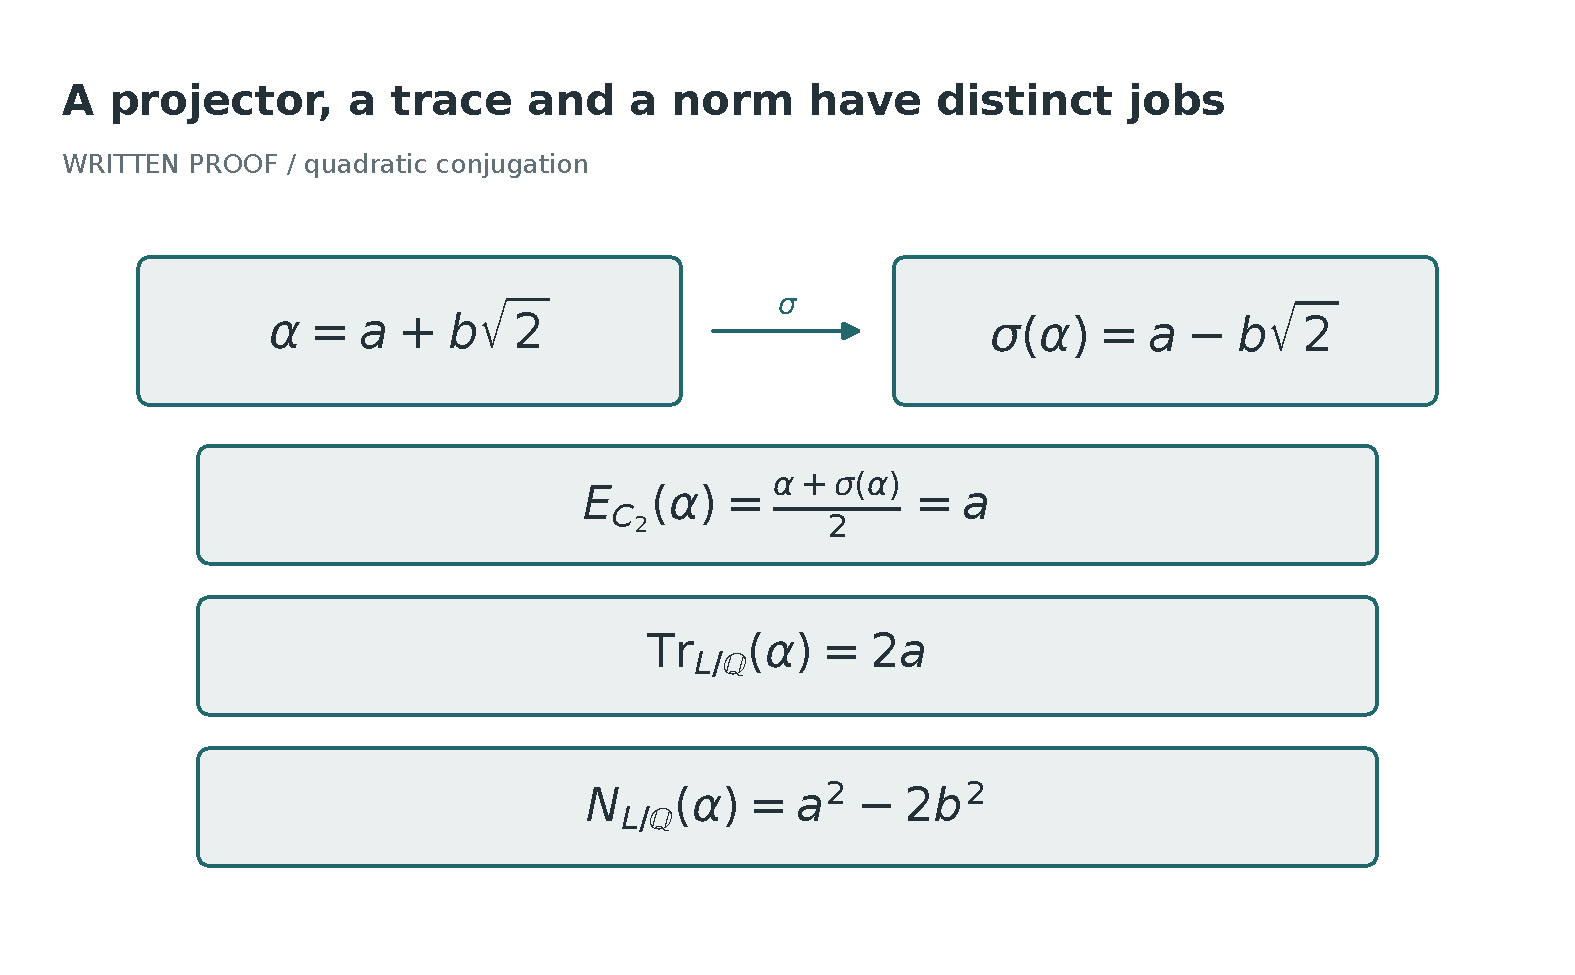
\includegraphics[width=0.96\linewidth]{../visual/figures/15_trace_norm.pdf}
\caption{In \(\Q(\sqrt2)\), averaging retains \(a\), trace retains \(2a\), and norm uses \(a^2-2b^2\). The multiplication and the discarded coordinate affect the norm even when the projected value stays fixed.}
\label{fig:b-trace-norm}
\end{figure}

\begin{claimboundary}
Subgroup averaging, ranks, compatibility, and normality have been proved for the regular module of every finite group. Classical Galois theory translates an already given field extension into that module language. The translation retains the field only when its multiplication and arithmetic base remain part of the object. A regular representation by itself supplies neither of them.
\end{claimboundary}

\addtocontents{toc}{\protect\newpage}
\chapter{A regular family and the specialization step}
\label{ch:regular-specialization}

The inverse Galois problem has a strong geometric route. First construct a family over \(\Q(t)\) with the desired finite Galois group. Then choose a rational parameter whose specialization retains the whole group. The second step is supplied by Hilbert irreducibility under precise hypotheses. The first step contains substantial arithmetic work. Treating the second step as automatic existence of the family would reverse the logical direction of the theorem.

\section{What regularity asks for}

Let \(t\) be transcendental over \(\Q\). A finite Galois extension \(F/\Q(t)\) is regular over \(\Q\) when \(\Q\) is algebraically closed in \(F\). Equivalently in the present characteristic zero setting,
\begin{equation}
 F\cap\overline{\Q}=\Q,
 \label{eq:b-regular-constants}
\end{equation}
inside an algebraic closure containing both fields. This condition excludes an extension obtained solely by enlarging the constants. It permits the family to remain connected over an algebraic closure of the constant field. The terminology and the implication from regular to ordinary realization over a Hilbertian base are documented in D\`ebes and Harbater \cite[Introduction]{DebesHarbater2021}.

If \(L/\Q\) is a nontrivial finite Galois extension, adjoining a dummy variable gives \(L(t)/\Q(t)\) with the same abstract group. It contains every element of \(L\) as an algebraic constant, so it is not regular. An ordinary realization therefore does not yield a regular one by this particular construction. The existence of a regular realization for every finite group is a stronger proposed input. This chapter uses no converse from ordinary realization to regular realization.

Regularity can be inspected only after the family is a field with a specified base. A matrix action depending on a symbol \(t\) does not by itself define \(F\). One needs equations or another construction of the extension, its connectedness, its arithmetic constant field, and the group of the full splitting field. These properties are part of the input to specialization.

\section{The exact specialization contract}

\begin{theorem}[Hilbert specialization, external input]
\label{thm:b-hilbert-specialization}
Let \(F/\Q(t)\) be a finite Galois field extension with group \(G\). After choosing a suitable model and excluding the finitely many zeros of a nonzero constraint polynomial, there are infinitely many rational values \(a\) for which a specialization has Galois group isomorphic to \(G\). In particular, an actual regular \(G\) extension of \(\Q(t)\) gives a \(G\) extension of \(\Q\).
\end{theorem}

This is the one parameter form of the checked Hilbert specialization contract. The source proof uses a primitive element for the entire Galois extension, a Hilbert subset preserving its irreducibility, and a localization avoiding coefficients, denominators, and discriminant zeros \cite[Theorem 2.6.3, Theorem 5.2.4 and Proposition 5.2.14]{DebesLectureNotes}. The regular consequence over \(\Q\) is also stated in the checked recent preprint \cite[Section 1.2]{HuangEtAl2026}. These are external theorem inputs. The present manuscript does not replace their proofs with a finite sample of parameter values.

The degree bookkeeping explains the conclusion. A primitive polynomial for \(F\) has degree \([F:\Q(t)]=|G|\). At suitable values its specialization remains irreducible of that degree. Away from the excluded model locus, specialization supplies a group inside the original \(G\). Preserving the full extension degree forces the specialized group to have \(|G|\) elements, hence to be the full group. A polynomial defining only one root field can have smaller degree, so preserving that polynomial's irreducibility alone is not this full degree argument.

\begin{corollary}[Conditional realization route]
\label{cor:b-regular-route}
For a prescribed finite group \(G\), a verified regular finite Galois extension \(F/\Q(t)\) with group \(G\), followed by Theorem~\ref{thm:b-hilbert-specialization}, proves an ordinary realization of \(G\) over \(\Q\).
\end{corollary}

\begin{proof}
Apply the external theorem to that extension, and choose one of the suitable rational parameters outside the finite excluded set. Its specialized field is the required finite Galois extension of \(\Q\).
\end{proof}

The theorem gives existence of suitable parameters. It does not identify every allowed parameter as suitable, nor does it automatically give a short search or a bound on the discriminant. A parameter outside the branch locus may still specialize to a smaller group. These are different questions: the model can be nonsingular at a value while the resulting polynomial acquires extra factorization over \(\Q\).

In several parameters, the excluded set is a proper algebraic locus and may be infinite. In one parameter, a nonzero polynomial has finitely many roots, which is why the finite exceptional set wording is appropriate here. The base \(\Q\) is also essential to the source contract. Characteristic zero by itself does not imply Hilbert irreducibility. For instance, over \(\C\) every specialization of a nonconstant irreducible polynomial in \(X\) splits into linear factors, so the required retention of a degree greater than one fails.

\begin{figure}[tbp]
\centering
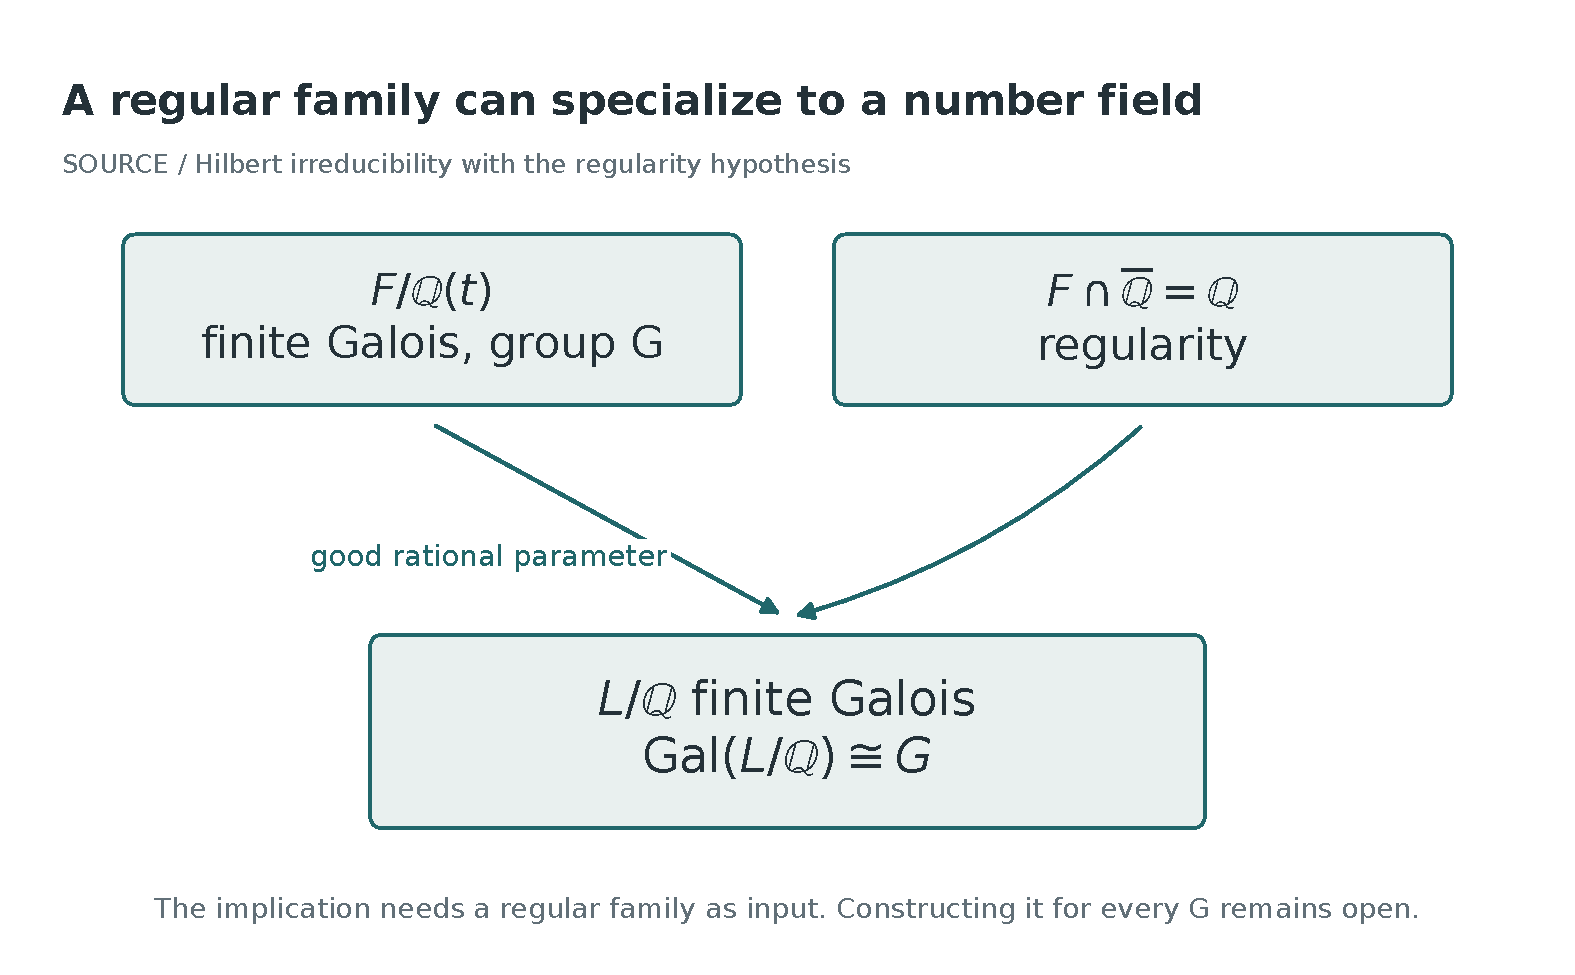
\includegraphics[width=0.96\linewidth]{../visual/figures/16_regular_specialization.pdf}
\caption{The specialization theorem starts with a verified arithmetic family. The suitable rational parameter belongs to a Hilbert subset and avoids the chosen model's exceptional values. Both conditions appear in the inference to a field over \(\Q\).}
\label{fig:b-regular-specialization}
\end{figure}

\section{A cubic toy that changes group}

The polynomial
\begin{equation}
 f_t(X)=X^3-t
 \label{eq:b-cubic-family}
\end{equation}
is a small exact example of what can happen under specialization. It is used here to study changes in the splitting field group. Its generic splitting field is not a regular extension of \(\Q(t)\), a fact established below.

At \(t=2\), the polynomial \(X^3-2\) is irreducible by Eisenstein at the prime \(2\). Let \(\alpha=\sqrt[3]{2}\) be the real root and let \(\zeta\) be a primitive cube root of unity. The splitting field is
\[
 L_2=\Q(\alpha,\zeta).
\]
The real field \(\Q(\alpha)\) has degree three. It cannot contain the nonreal element \(\zeta\). Adjoining \(\zeta\), whose minimal polynomial is \(X^2+X+1\), therefore doubles the degree. The splitting field has degree six and its faithful action on the three roots identifies its group with \(S_3\). Equivalently, the discriminant is \(-27\cdot2^2=-108\), which is not a rational square. The classical irreducible cubic criterion is checked in Milne \cite[Proposition 4.5 and Example 4.7]{Milne2022}.

At \(t=1\),
\[
 X^3-1=(X-1)(X^2+X+1).
\]
The splitting field is \(\Q(\zeta)\), of degree two, with group \(C_2\). The discriminant \(-27\) is nonzero, so this is an unbranched parameter for the simple discriminant test, yet the group has dropped from \(S_3\). At \(t=0\), the polynomial becomes \(X^3\), with a repeated root, and its splitting field is simply \(\Q\). That value lies on the discriminant zero locus. Thus the toy separates a singular degeneration from a nonsingular group drop.

The generic splitting field also has group \(S_3\). To prove this without an experimental inference, take a transcendental \(u\) and put \(t=u^3\). The polynomial \(X^3-t\) is Eisenstein at the prime \(t\) in \(\Q[t][X]\), hence irreducible over \(\Q(t)\). Its root field is \(\Q(u)\), and the splitting field is \(\Q(u,\zeta)\). The only elements of \(\Q(u)\) algebraic over \(\Q\) lie in \(\Q\). Indeed, if a nonconstant rational function \(v(u)\) were algebraic over \(\Q\), clearing the equation defining \(v\) would make \(u\) algebraic over \(\Q(v)\), contradicting its transcendence. Hence \(\zeta\notin\Q(u)\). The generic extension again has degree six and group \(S_3\).

However, its constant field contains \(\Q(\zeta)\), so it violates \eqref{eq:b-regular-constants}. It cannot serve as the worked regular input of Corollary~\ref{cor:b-regular-route}. The valid conclusions are the three specialization computations and the explicit generic group calculation. The general specialization theorem also admits nonregular finite Galois inputs under its stated model hypotheses, but their specializations need not give infinitely many distinct field isomorphism classes. A constant extension illustrates why suitable parameter values and distinct extensions should not be identified without an additional argument.

\begin{figure}[tbp]
\centering
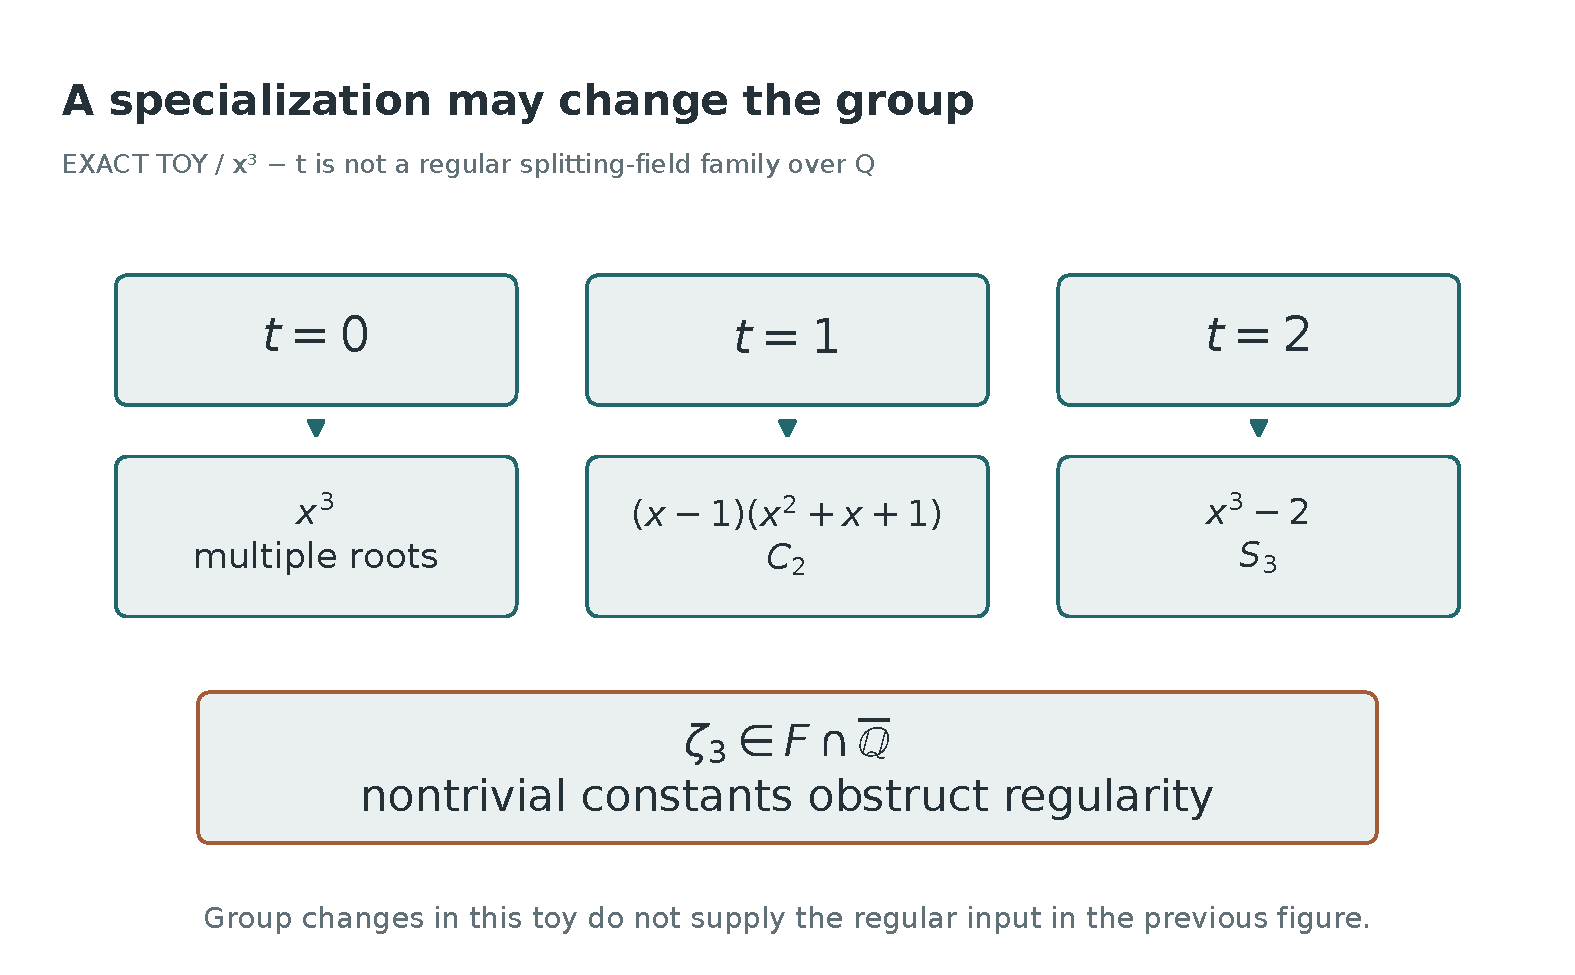
\includegraphics[width=0.96\linewidth]{../visual/figures/17_parameter_bad.pdf}
\caption{The specialization toy \(X^3-t\) has group \(S_3\) at \(t=2\), group \(C_2\) at the nonsingular value \(t=1\), and trivial splitting field at \(t=0\). Its generic splitting field contains \(\zeta_3\), so this is not a regular family over \(\Q\).}
\label{fig:b-parameter-toy}
\end{figure}

\section{Geometric existence and arithmetic descent}

A construction over \(\C(t)\) has a different base from one over \(\Q(t)\). Even if it comes from an exact complex cover with the intended group, the construction still needs an arithmetic model over \(\Q\), together with compatible equations and descent data. An action on its geometric fibers does not by itself prove that this model exists over the smaller base.

The elementary constant example already displays the issue. The equation \(X^3-t\) has cyclic splitting field over \(\C(t)\), since \(\zeta_3\) is in the base. Over \(\Q(t)\), its splitting field has group \(S_3\), with an extra arithmetic action on that constant. Passing between bases can change the group being discussed. For a regular arithmetic family, one must verify the stated arithmetic group and the absence of enlarged constants, rather than assigning the geometric group to both settings by notation.

This is where the packet language can record a useful obligation. A geometric construction may organize branch behavior, group actions, and local charts. An arithmetic descent claim asks that its chart transitions and coefficients arise from an effective object over \(\Q\). A specialization claim then starts from that object. Keeping the two steps separate prevents a valid complex construction from being promoted into an unsupported rational realization.

\begin{openproblem}
For the general regular route, the missing input is a verified regular \(G\) extension over \(\Q(t)\) for each prescribed finite group \(G\). Hilbert specialization applies after that input has been constructed. A complex cover, a regular module, or a compatible system of projectors does not establish the required arithmetic descent by itself.
\end{openproblem}

\chapter{Embedding problems and the lift that must be proper}
\label{ch:embedding-problems}

An embedding problem makes the realization obstruction relative. Suppose one finite Galois extension has already been found. Can it be enlarged so that a prescribed extension of its group appears as the full new Galois group? This asks for more than constructing an abstract extension of finite groups. The new group must be reached by a continuous quotient of the absolute Galois group, and the quotient must respect the existing field.

\section{The diagram and its fields}

Fix an algebraic closure \(\overline\Q\), and write
\[
 G_{\Q}=\Gal(\overline\Q/\Q)
\]
with its Krull topology. For a finite Galois subfield \(L\subset\overline\Q\), restriction supplies a continuous epimorphism \cite[Proposition 7.7]{Milne2022}
\[
 \rho:G_{\Q}\longrightarrow G=\Gal(L/\Q).
\]
Now specify an exact sequence of finite groups
\begin{equation}
 1\longrightarrow N\longrightarrow E\overset{\pi}{\longrightarrow}G\longrightarrow1.
 \label{eq:b-group-extension}
\end{equation}
The finite targets carry the discrete topology. A solution is a continuous homomorphism
\begin{equation}
 \widetilde\rho:G_{\Q}\longrightarrow E,
 \qquad \pi\circ\widetilde\rho=\rho.
 \label{eq:b-lift-equation}
\end{equation}
It is a weak solution when this equation holds, and a proper solution when \(\widetilde\rho\) is also surjective.

Continuity is part of the definition. For a finite discrete target it makes the kernel open. The fixed field of that kernel is therefore a finite Galois extension of \(\Q\), with group equal to the image of the map. These facts belong to the classical absolute Galois correspondence \cite[Theorem 7.13]{Milne2022}. They explain why a homomorphism without the continuity hypothesis is not the required arithmetic certificate.

Let \(J=\widetilde\rho(G_{\Q})\leq E\). Even a weak solution satisfies \(\pi(J)=G\), since \(\rho\) is onto. The inclusion \(\ker\widetilde\rho\subseteq\ker\rho\) gives a finite Galois field \(M\) containing \(L\). Its group is \(J\), rather than necessarily \(E\). Properness makes the exact arithmetic tower
\[
 \Gal(M/\Q)\cong E,
 \qquad \Gal(M/L)\cong N,
 \qquad \Gal(L/\Q)\cong G.
\]
The quotient map in this tower must be the specified \(\pi\) under these identifications.

\begin{figure}[tbp]
\centering
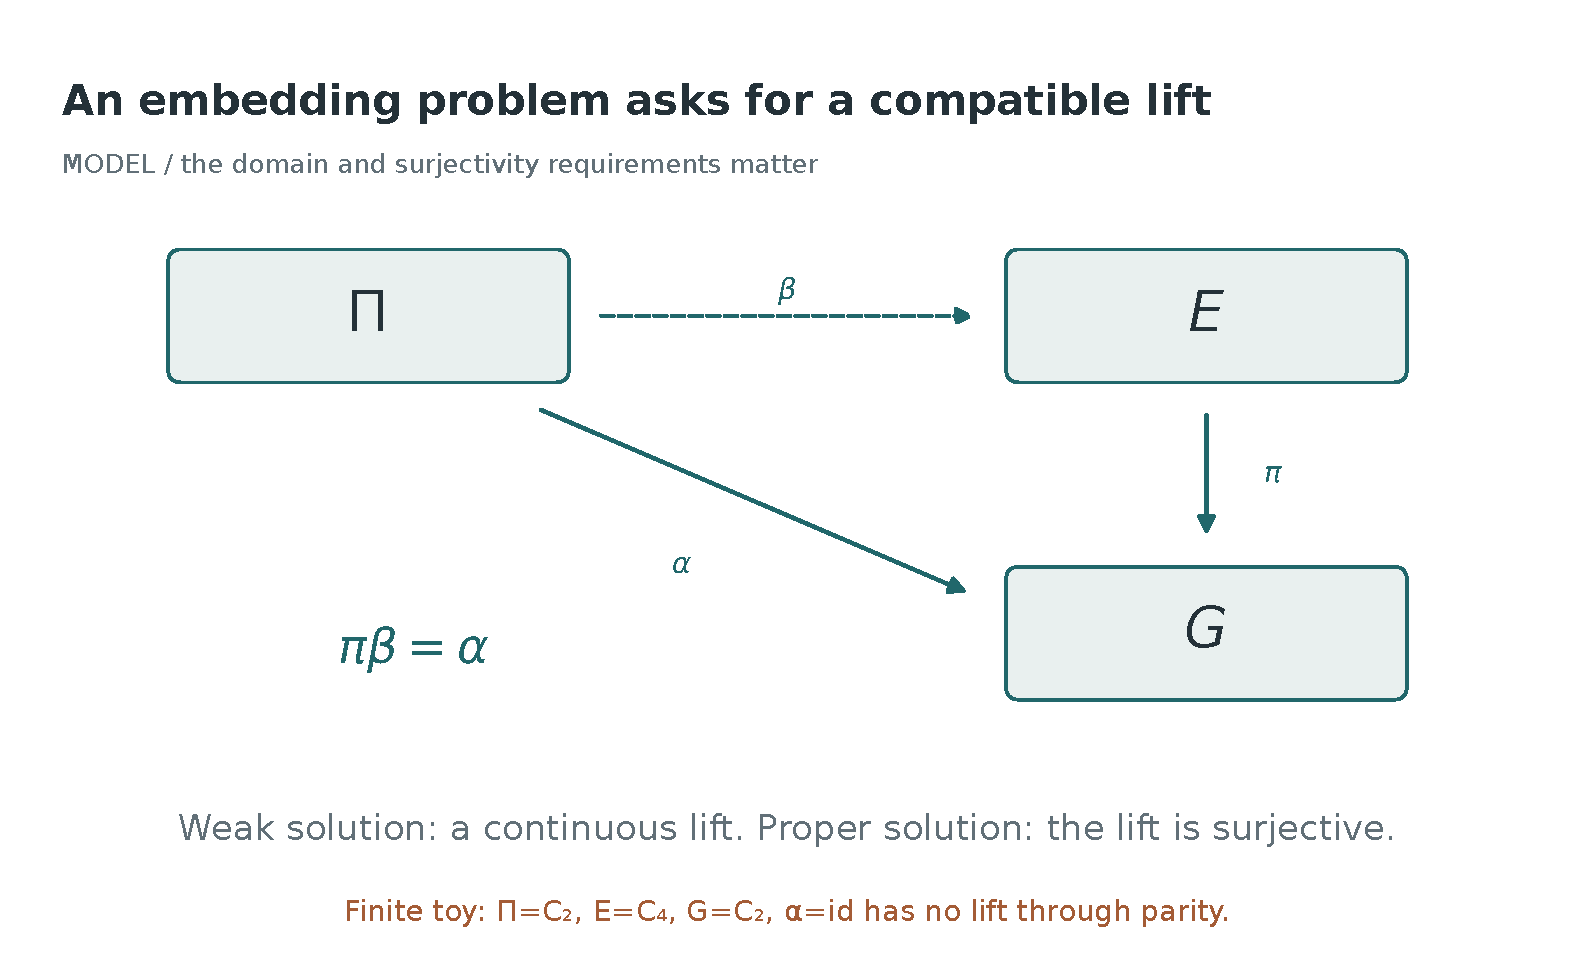
\includegraphics[width=0.96\linewidth]{../visual/figures/18_embedding_problem.pdf}
\caption{An embedding problem fixes the quotient map \(\pi:E\to G\) and the existing arithmetic quotient \(\rho:G_{\Q}\to G\). The lift must be continuous, must make the triangle commute, and must be surjective to be proper.}
\label{fig:b-embedding-problem}
\end{figure}

\section{A finite no lift toy}

The following example is an exact finite group calculation. Its domain is the finite group \(C_2\), rather than \(G_{\Q}\). It is useful because it isolates an obstruction to lifting a relation.

\begin{example}[The identity of \(C_2\) does not lift to \(C_4\)]
\label{ex:b-no-lift}
Use additive notation and take
\[
 \Gamma=\Z/2\Z,
 \quad E=\Z/4\Z,
 \quad G=\Z/2\Z,
 \quad \pi(x)=x\bmod2,
 \quad \rho=\operatorname{id}_{\Gamma}.
\]
If \(\widetilde\rho:\Gamma\to E\) were a lift, the image \(y\) of the nonzero element would satisfy \(\pi(y)=1\), so \(y\) would be \(1\) or \(3\) modulo four. But the relation \(1+1=0\) in \(\Gamma\) forces \(2y=0\) in \(E\), which holds only for \(y=0\) or \(2\). No such lift exists.
\end{example}

The surjection \(C_4\to C_2\) is perfectly valid, and each element of \(C_2\) has a preimage. The failure occurs when the preimages must respect the domain's group law. Lifting individual elements is therefore weaker than lifting the homomorphism. An arithmetic construction must respect all relations and its continuity requirements at once.

This toy is not a counterexample to solvability of an absolute Galois embedding problem with the same finite targets. Its proof uses the order two relation in the chosen finite domain. The absolute Galois group is a different domain, and an arithmetic quotient may be reached through elements and relations that are absent from this toy. The example supplies a precise warning about an invalid inference, not a general arithmetic impossibility theorem.

\section{A split lift can still be weak}

An extension splits when \(\pi\) has a homomorphic section \(s:G\to E\). For such a section, \(s\circ\rho\) is automatically a continuous weak solution: \(\rho\) is continuous by hypothesis, \(s\) is continuous between finite discrete groups, and \(\pi s\rho=\rho\). Its image is \(s(G)\). If the kernel \(N\) is nontrivial, this image has order \(|G|<|E|\), so that particular solution is not proper.

\begin{example}[The kernel is missed in a direct product]
\label{ex:b-split-weak}
Take \(E=N\times G\) with \(\pi(n,g)=g\). The section \(s(g)=(1,g)\) gives
\[
 \widetilde\rho_0(\gamma)=(1,\rho(\gamma)).
\]
Its image is \(\{1\}\times G\). It reaches every element of the desired quotient, but reaches none of the nonidentity elements of \(N\times\{1\}\). With the finite toy \(N=G=\Gamma=C_2\) and \(\rho\) the identity, the image has two elements while \(E\) has four. All lift equations hold, and properness fails.
\end{example}

\begin{proposition}[Exact kernel coverage criterion]
\label{prop:b-kernel-coverage}
Let \(\Gamma\) be any group, let \(\rho:\Gamma\to G\) be onto, and let \(\widetilde\rho:\Gamma\to E\) be a homomorphic lift through \eqref{eq:b-group-extension}. Then \(\widetilde\rho\) is onto if and only if
\begin{equation}
 \widetilde\rho(\ker\rho)=N.
 \label{eq:b-kernel-coverage}
\end{equation}
\end{proposition}

\begin{proof}
Every image of \(\ker\rho\) lies in \(N\). If \(\widetilde\rho\) is onto, every \(n\in N\) has a preimage \(\gamma\), and \(\rho(\gamma)=\pi(n)=1\), proving the equality. Conversely, assume the equality and take \(e\in E\). Surjectivity of \(\rho\) gives \(\gamma\) with \(\rho(\gamma)=\pi(e)\). Then \(e\widetilde\rho(\gamma)^{-1}\in N\). By the hypothesis it equals \(\widetilde\rho(\delta)\) for some \(\delta\in\ker\rho\). Hence \(e=\widetilde\rho(\delta\gamma)\), proving surjectivity.
\end{proof}

This criterion gives an exact remaining task after a weak solution is found. The quotient has already been covered. Properness asks whether the arithmetic kernel supplies the full additional group. A computation of the quotient action alone cannot answer that question.

For a direct product, a candidate lift has the form \((\eta,\rho)\), where \(\eta:\Gamma\to N\) is a homomorphism. Even surjectivity of both coordinates does not automatically imply surjectivity of the pair. If \(\Gamma=N=G=C_2\) and both maps are the identity, their combined image is the diagonal subgroup of order two. Proposition~\ref{prop:b-kernel-coverage} locates the failure: the kernel of \(\rho\) is trivial and supplies no nontrivial kernel element.

\begin{figure}[tbp]
\centering
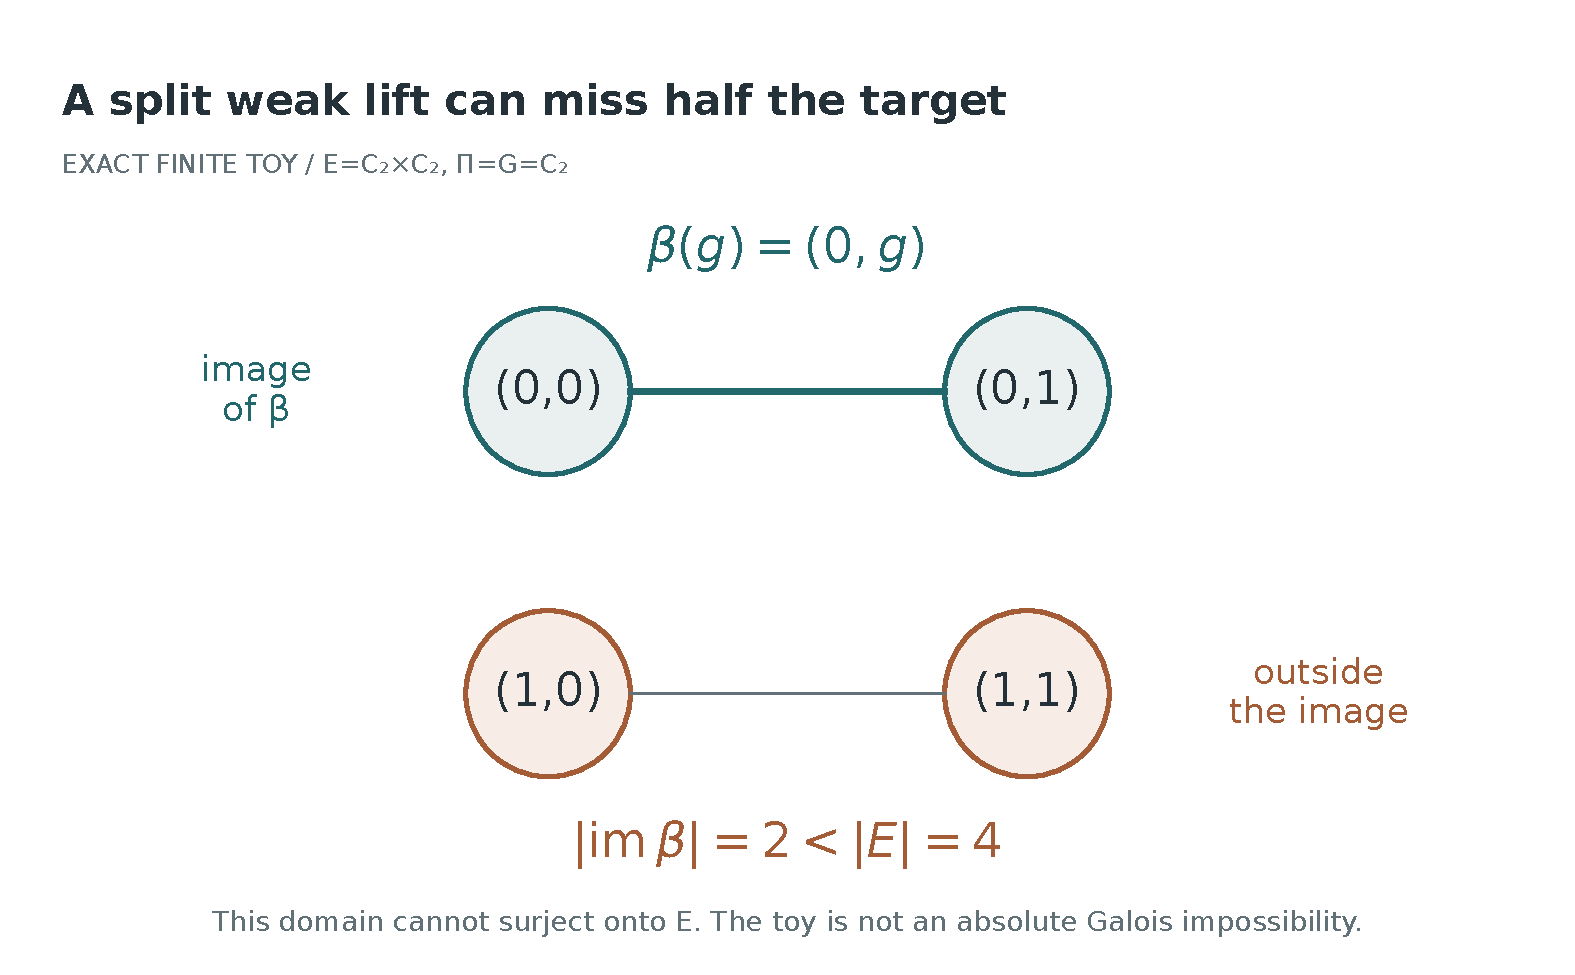
\includegraphics[width=0.96\linewidth]{../visual/figures/19_weak_proper.pdf}
\caption{A weak solution can cover the quotient while missing the extension kernel. Properness requires exactly \(\widetilde\rho(\ker\rho)=N\), in addition to the commuting lift equation. The finite split example illustrates this distinction.}
\label{fig:b-weak-proper}
\end{figure}

\FloatBarrier
\section{The relation defect of a chosen section}

A set theoretic section may select preimages without being a homomorphism. Its failure to preserve products is an exact defect. To state the calculation cleanly, assume here that \(N\) is central in \(E\). Centrality makes \(N\) abelian. Choose a section \(s:G\to E\) with \(s(1)=1\), and define
\begin{equation}
 c(g,h)=s(g)s(h)s(gh)^{-1}\in N.
 \label{eq:b-section-defect}
\end{equation}
Associativity in \(E\) gives
\begin{equation}
 c(g,h)c(gh,k)=c(h,k)c(g,hk),
 \label{eq:b-cocycle-law}
\end{equation}
because central elements can be moved past the section values. The normalized identities are \(c(1,g)=c(g,1)=1\). Thus the defect is a central two cocycle, with its law proved by the group multiplication itself.

\begin{proposition}[Explicit central lift equation]
\label{prop:b-central-lift}
For a homomorphism \(\rho:\Gamma\to G\), a lift has the form
\begin{equation}
 \widetilde\rho(\gamma)=u(\gamma)s(\rho(\gamma)),
 \qquad u(\gamma)\in N.
 \label{eq:b-corrected-section}
\end{equation}
It is a homomorphism if and only if \(u(1)=1\) and
\begin{equation}
 u(\gamma\delta)
 =u(\gamma)u(\delta)c(\rho(\gamma),\rho(\delta))
 \quad(\gamma,\delta\in\Gamma).
 \label{eq:b-correction-equation}
\end{equation}
For a topological domain and finite targets, the lift is continuous if and only if \(u\) is continuous, provided \(\rho\) is continuous.
\end{proposition}

\begin{proof}
Any lift differs from \(s\rho\) by a unique element of the kernel, giving \eqref{eq:b-corrected-section}. Centrality and \eqref{eq:b-section-defect} give
\[
 \widetilde\rho(\gamma)\widetilde\rho(\delta)
 =u(\gamma)u(\delta)c(\rho(\gamma),\rho(\delta))s(\rho(\gamma\delta)).
\]
Comparison with the expression for \(\widetilde\rho(\gamma\delta)\) proves the equivalence. The identity condition makes the identity map correctly. Since a map between finite discrete sets is continuous, \(s\rho\) is continuous whenever \(\rho\) is. The equation relating \(u\) and \(\widetilde\rho\) then proves both directions of the continuity assertion.
\end{proof}

This proposition states the obstruction without assuming it disappears. A successful correction \(u\) removes the pulled back defect in the stated multiplicative convention. In cohomological terminology this is the triviality of the corresponding pulled back class. Such triviality needs a proof for the actual arithmetic quotient and kernel action. For a noncentral kernel, conjugation introduces a nontrivial action and changes the correction equation. The central formula cannot be used unchanged there.

The finite \(C_4\) example also appears in these coordinates. In additive notation select \(s(0)=0\), \(s(1)=1\). The defect at \((1,1)\) is \(2\) modulo four. A correction \(u(1)\) must be in the kernel \(\{0,2\}\). Equation~\eqref{eq:b-correction-equation} then becomes
\[
 0=2u(1)+2\pmod4,
\]
which is impossible. This reproduces the order obstruction using a relation defect. It is an exact finite computation and an exact finite proof. It supplies no assertion that an analogous class always vanishes or always persists over \(G_{\Q}\).

\section{What closes an arithmetic embedding problem}

For a specific arithmetic problem, the required certificate has three layers. First the starting map \(\rho\) must come from the declared finite Galois extension. Second a continuous lift must solve the exact relation equation for the chosen group extension, with all actions and descent data specified. Third the image must be the full group \(E\), equivalently the arithmetic kernel must cover \(N\).

A projector construction can faithfully encode the finite targets and their quotient action. It can also keep a residual for a failed relation or a missed kernel direction. That is useful evidence about the construction. It becomes an arithmetic existence proof only when the corrected data define the required continuous quotient and its finite fixed field. The source theorem realizing finite solvable groups over \(\Q\) is a substantial external existence result \cite[Theorem 1]{SchmidtWingberg1998}. It cannot be substituted for an unchecked claim that every specified embedding problem, with every prescribed local condition, has a proper solution.

The same care applies to descent. Matching a finite collection of matrices can prove a compatibility identity within their realized vector spaces. Effective descent requires the identity to be part of a complete object over the intended field, including its coefficients and multiplication. A local chart repair may remove one visible defect while leaving another arithmetic obstruction. The resolved language helps by naming those separate obligations rather than treating a zero matrix residual as the end of every existence problem.

\begin{claimboundary}
The finite lift obstruction, the split weak lift, the kernel coverage criterion, and the central correction equation have complete arguments in this chapter. They organize the remaining arithmetic task. They do not prove that every embedding problem over \(G_{\Q}\) has a proper solution, and they do not close the unrestricted inverse Galois conjecture.
\end{claimboundary}
